\documentclass[
  % all of the below options are optional and can be left out
  % course name (default: 2IL50 Data Structures)
  course = {{16-720B Computer Vision}},
  % quartile (default: 3)
  quartile = {{1}},
  % assignment number/name (default: 1)
  assignment = 2-Bag\ of \ Visual\ Words,
  % student name (default: Some One)
  name = {{Kangle Deng}},
  % student number, NOT S-number (default: 0123456)
  % studentnumber = {{0123456 ; 0314159}},
  % student email (default: s.one@student.tue.nl)
  email = {{kangled@andrew.cmu.edu}},
  % first exercise number (default: 1)
  firstexercise = 1
]{aga-homework}

\usepackage{url}

\begin{document}
\section{Representing the World with Visual Words}
\subsection{Extracting Filter Responses}
\noindent \textbf{Q1.1.1}
\begin{itemize}
    \item \textbf{Smoothing:} Gaussian.
    \item \textbf{Edge Detector:} Laplacian of Gaussian, derivative of Gaussian in the $x$ direction, derivative of Gaussian in the $y$ direction.
\end{itemize}

Multiple scales of filters are meant to detect objects (here edges) of different scales (here width of edges).

\noindent \textbf{Q1.1.2} 

Figure \ref{fig:hw2_q112} is the result.
\begin{figure}
    \centering
    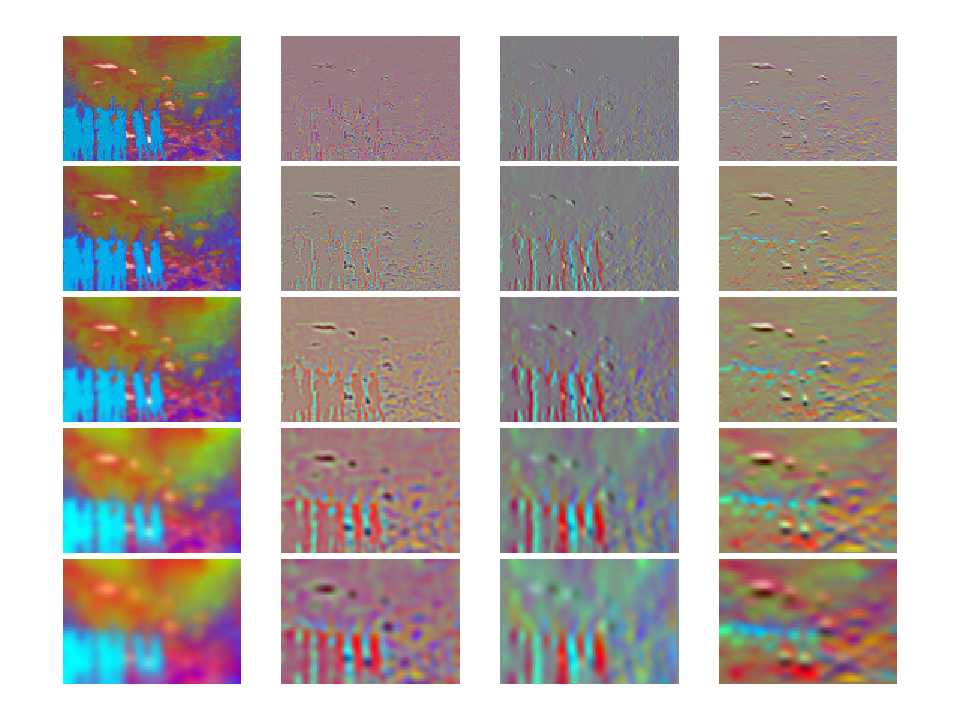
\includegraphics{CV/fig/hw2/Q112.pdf}
    \caption{Q1.1.2: filter responses}
    \label{fig:hw2_q112}
\end{figure}

\subsection{Creating Visual Words}
\noindent \textbf{Q1.2.1}

I choose $k$ as 0.05. Figure \ref{fig:hw2_q121} is the result.

\begin{figure}
    \centering
    \subfigure{
        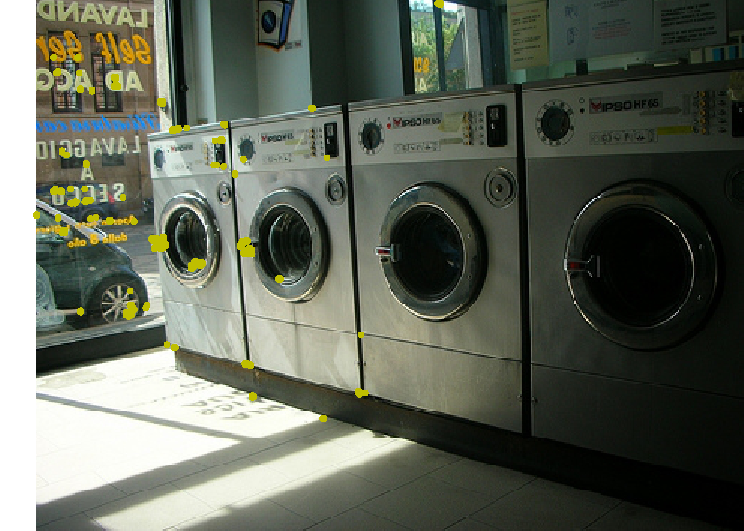
\includegraphics[width=.3\textwidth]{CV/fig/hw2/Q121-1.pdf}
    }
    \subfigure{
        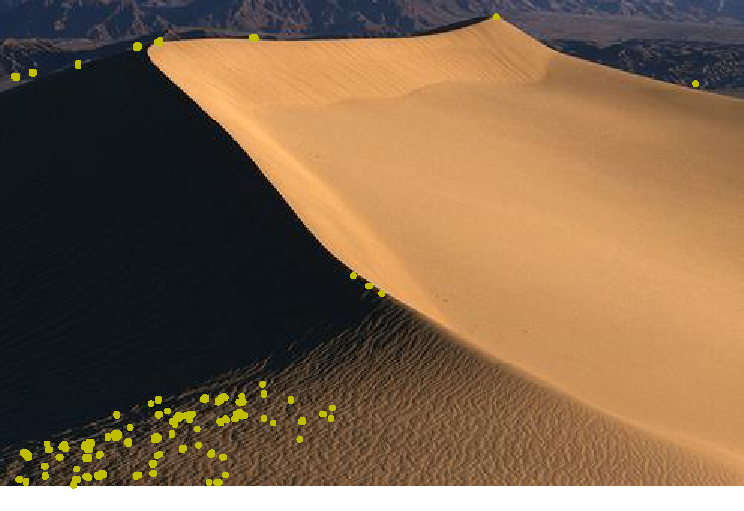
\includegraphics[width=.32\textwidth]{CV/fig/hw2/Q121-2.pdf}
    }
    \subfigure{
        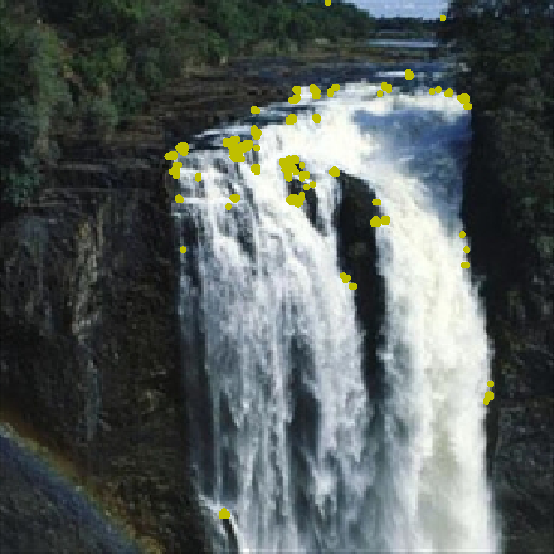
\includegraphics[width=.25\textwidth]{CV/fig/hw2/Q121-3.pdf}
    }
    \caption{Q1.2.1: Harris Corner Detector Results}
    \label{fig:hw2_q121}
\end{figure}

\noindent \textbf{Q1.2.2}

I choose $\alpha$ as 250, and $K$ as 200.

\noindent \textbf{Q1.3.1}

Figure \ref{fig:hw2_q131} is the result. The word boundaries sketch the outline of the objects (or segments of objects). This implies that those visual words somehow ``recognize'' different objects in those pictures.
\begin{figure}
    \centering
    \subfigure{
        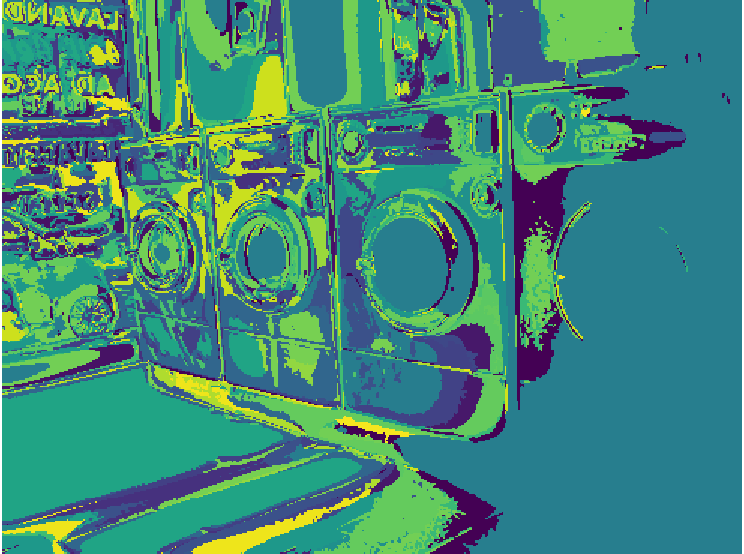
\includegraphics[width=.3\textwidth]{CV/fig/hw2/Q131/Q131-1.pdf}
    }
    \subfigure{
        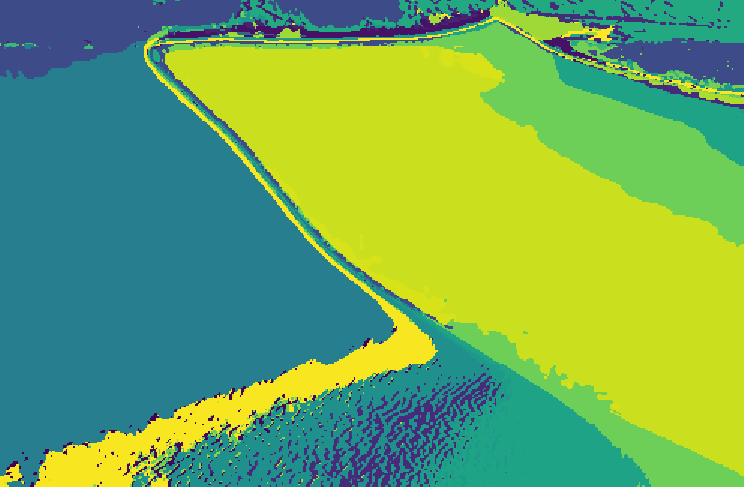
\includegraphics[width=.34\textwidth]{CV/fig/hw2/Q131/Q131-2.pdf}
    }
    \subfigure{
        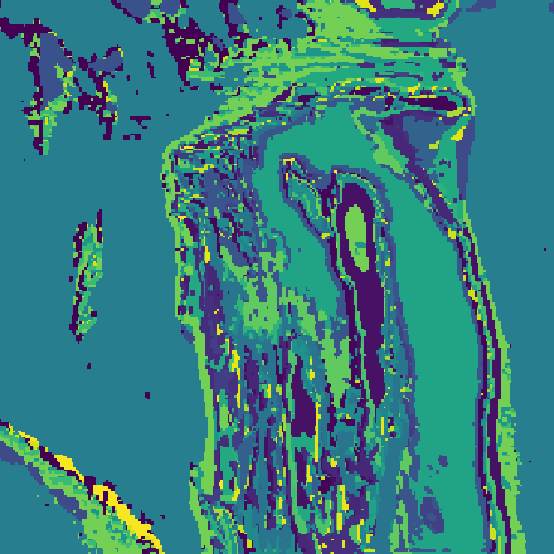
\includegraphics[width=.23\textwidth]{CV/fig/hw2/Q131/Q131-3.pdf}
    }
    \subfigure{
        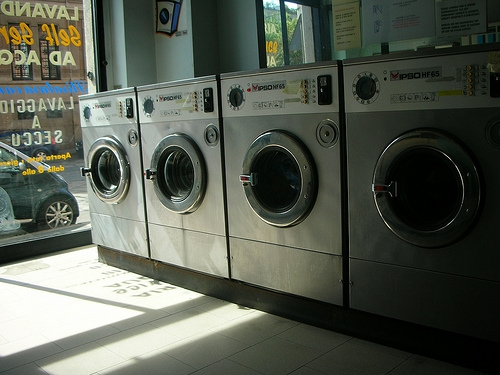
\includegraphics[width=.3\textwidth]{CV/fig/hw2/Q131/sun_addinpsdbmiewyvc.jpg}
    }
    \subfigure{
        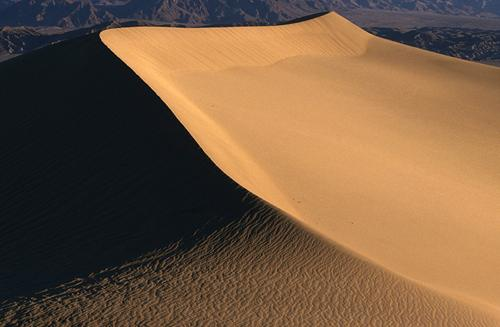
\includegraphics[width=.34\textwidth]{CV/fig/hw2/Q131/sun_abdulxymarqnjwgh.jpg}
    }
    \subfigure{
        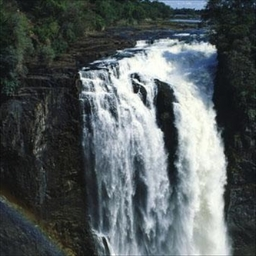
\includegraphics[width=.23\textwidth]{CV/fig/hw2/Q131/sun_alheovotlhwqzvmo.jpg}
    }
    \caption{Q1.3.1: Visual Words Results: The word boundaries sketch the outline of the objects (or segments of objects). This implies that those visual words somehow ``recognize'' different objects in those pictures.}
    \label{fig:hw2_q131}
\end{figure}

\section{Building a Recognition System}
\subsection{Extracting Features}
\noindent\textbf{Q2.1.1}

Figure \ref{fig:hw2_q211} is the histogram of the image aquarium/sun aztvjgubyrgvirup.jpg.

\begin{figure}
    \centering
    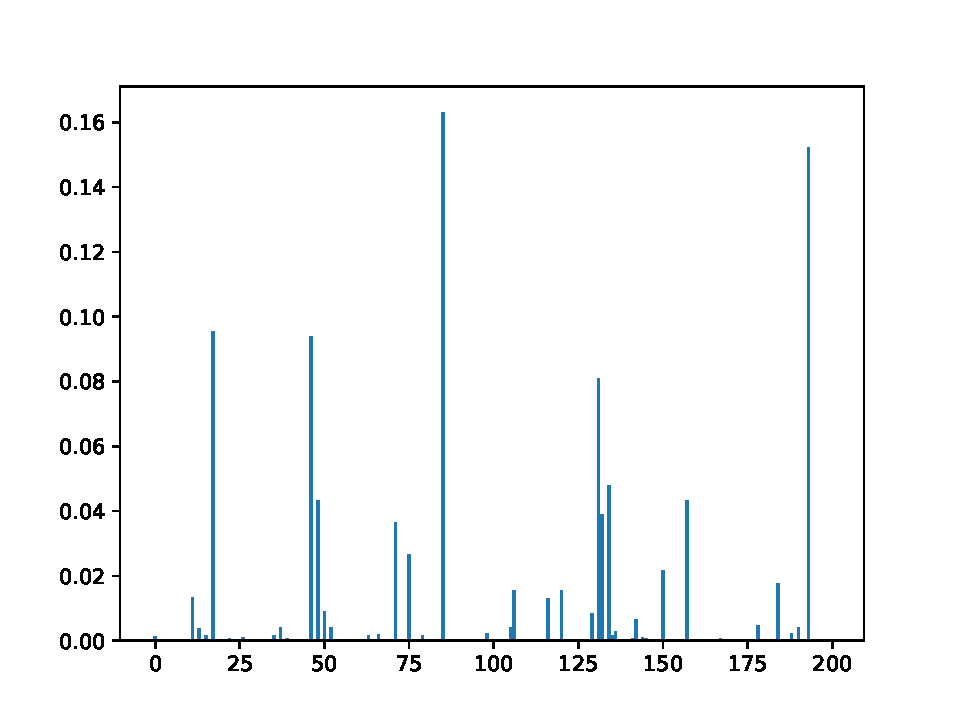
\includegraphics{CV/fig/hw2/Q211.pdf}
    \caption{Q2.1.1: Histogram}
    \label{fig:hw2_q211}
\end{figure}

\subsection{Multi-resolution: Spatial Pyramid Matching}
\noindent\textbf{Q2.2.1}

I use $K = 200, L = 2$. So the feature dim is $4200$.

\subsection{Comparing images}
\noindent\textbf{Q2.3.1}

Please see my code.

\subsection{Building a Model of the Visual World}
\noindent\textbf{Q2.4.1}
I implement it in a parallel way. Please see my code.

\section{Quantitative Evaluation}
\subsection{Calculating confusion matrix}
\noindent \textbf{Q3.1.1}

The confusion matrix is as follow:
\begin{verbatim}
[[14.  0.  0.  0.  0.  0.  0.  0.]
 [ 1. 12.  1.  1.  0.  2.  1.  0.]
 [ 0.  0. 16.  1.  5.  0.  0.  3.]
 [ 0.  3.  1. 13.  0.  1.  0.  8.]
 [ 1.  1.  1.  0.  9.  1.  0.  0.]
 [ 0.  1.  0.  1.  8. 12.  2.  0.]
 [ 1.  3.  1.  0.  2.  1. 12.  1.]
 [ 0.  1.  1.  2.  2.  0.  2. 11.]]
\end{verbatim}

The accuracy is $61.875\%$.

\noindent \textbf{Q3.1.2}

\textbf{Highway} and \textbf{Laundromat} are 2 classes that are the most difficult to classify. For Highway, there are $30.8\%$ of the test data mis-classified as Windmill. Most of those mis-classified images (see Figure \ref{fig:hw2_q312-highway}) are country-roads that are surrounded by trees and woods. On the other hand, trees and woods are also very common in many of the windmill scenes. So many of those Highways (country-roads) are mis-classified as Windmills. For Laundromat, there are $33.3\%$ of the test data mis-classified as Kitchen. This is because both laundromats and kitchens are normal indoor scenes. So they share a lot of indoor common objects: windows, pillars, tables, and 
ceramic tiles (see Figure \ref{fig:hw2_q312-laundromat}).

In conclusion, most of the mis-classifications are because of the shared features in different scenes.

\begin{figure}
    \centering
    \subfigure{
        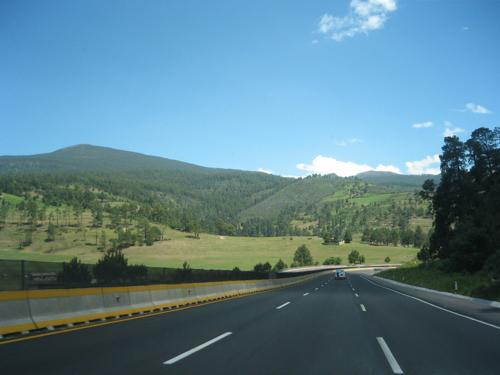
\includegraphics[width=.32\textwidth]{CV/fig/hw2/Q312/highway/sun_bghvacyqcglzhzaf.jpg}
    }
    \subfigure{
        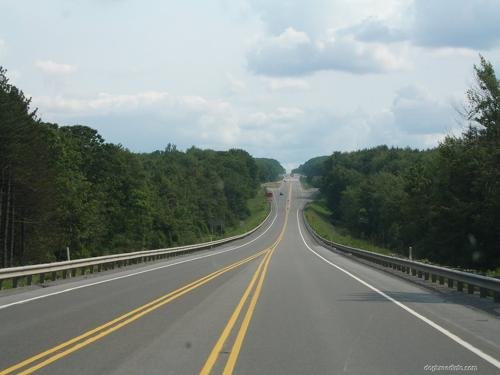
\includegraphics[width=.32\textwidth]{CV/fig/hw2/Q312/highway/sun_boijgyvghsntwyie.jpg}
    }
    \subfigure{
        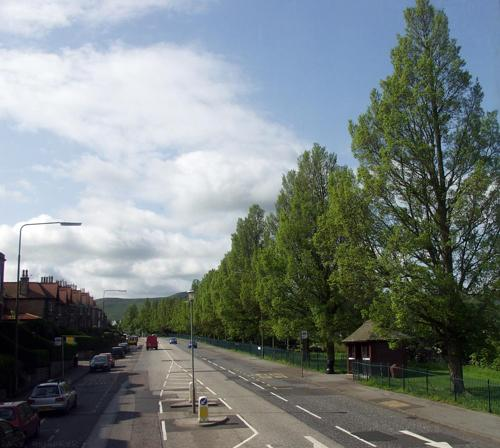
\includegraphics[width=.27\textwidth]{CV/fig/hw2/Q312/highway/sun_bsqoowlelpxyjkyt.jpg}
    }
    \caption{Q3.1.2: Highways mis-classified as Windmills}
    \label{fig:hw2_q312-highway}
\end{figure}

\begin{figure}
    \centering
    \subfigure{
        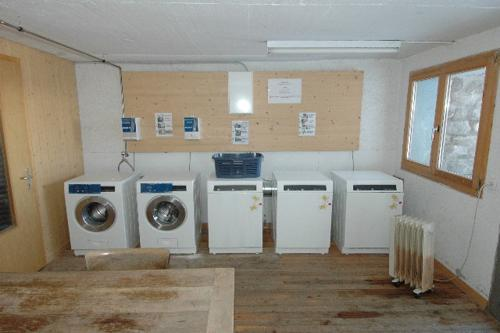
\includegraphics[width=.34\textwidth]{CV/fig/hw2/Q312/laundromat/sun_aiewbfesvvdzrhei.jpg}
    }
    \subfigure{
        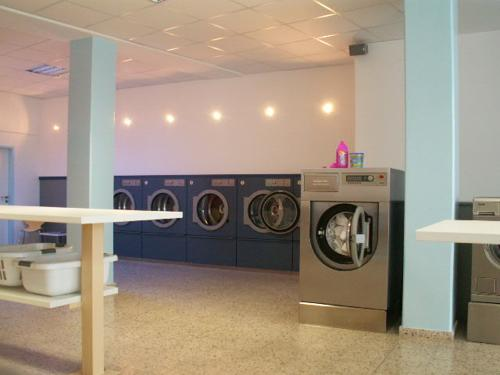
\includegraphics[width=.31\textwidth]{CV/fig/hw2/Q312/laundromat/sun_anptqnweaizqrczm.jpg}
    }
    \subfigure{
        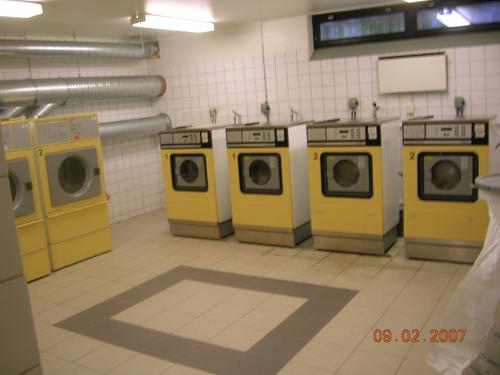
\includegraphics[width=.31\textwidth]{CV/fig/hw2/Q312/laundromat/sun_awytptirbthbwszg.jpg}
    }
    \caption{Q3.1.2: Laundromat mis-classified as Kitchen}
    \label{fig:hw2_q312-laundromat}
\end{figure}

% 1: 6 / 18
% 2: 9 / 25
% 3: 13 / 26 highway
% 4: 4 / 13
% 5: 12 / 24 laundromat
% 6: 9 / 21 waterfall
% 7: 8 / 19 windmill

\noindent \textbf{Q3.1.3}

From Figure \ref{fig:hw2_q121}, I find that there are some redundant keypoints and some other keypoints are not identified. So I increase the Harris Corner threshold $k$ from $0.05$ to $0.06$, thus filtering away some redundant points.

From Figure \ref{fig:hw2_q131}, some object boundaries are not perfectly recognized. I increase $\alpha$ from $250$ to $500$ to include more samples in the building of dictionary, thus making visual words more precise.

Finally, $K = 200, L = 2,$ which I do not change.

The confusion matrix is:
\begin{verbatim}
[[13.  0.  0.  1.  0.  0.  0.  0.]
 [ 0. 16.  0.  0.  0.  1.  1.  0.]
 [ 0.  0. 19.  1.  2.  0.  1.  2.]
 [ 0.  2.  2. 14.  0.  1.  2.  5.]
 [ 2.  0.  2.  0.  8.  1.  0.  0.]
 [ 1.  1.  0.  0. 10. 11.  1.  0.]
 [ 0.  5.  1.  0.  3.  1. 11.  0.]
 [ 0.  1.  2.  2.  1.  0.  2. 11.]]
\end{verbatim}
And the accuracy is $64.375\%$. The trained system is saved as $trained\_system\_tuned.npz$, check $custom.py$ to run it.

\noindent \textbf{Q3.1.4}

I implement IDF and use it to weight the BOW features. However, the accuracy drops to $52.5\%$. The confusion matrix is as follow:

\begin{verbatim}
[[13.  0.  0.  0.  0.  1.  0.  0.]
 [ 0. 16.  0.  0.  0.  1.  0.  1.]
 [ 0.  0.  9.  1.  5.  2.  1.  7.]
 [ 1.  1.  1. 12.  0.  2.  3.  6.]
 [ 0.  0.  1.  0.  9.  3.  0.  0.]
 [ 2.  3.  3.  0.  6.  8.  0.  2.]
 [ 1.  7.  1.  1.  2.  0.  8.  1.]
 [ 0.  2.  3.  3.  0.  1.  1.  9.]]
\end{verbatim}

The use of IDF alleviates the negative effect by the shared features of different classes, which we discuss in \textbf{Q3.1.2}. For example, there are less highways mis-classified as windmills, and less laundromats mis-classified as kitchens. In spite of those positive effect that IDF brings, it also raises some problems that it actually puts more weights on those unique noises (not appearing in other images but does no help to classification).

The IDF results is saved as $IDF.npy$.

\section{Deep Learning Features - An Alternative to ``Bag of Words''}
\subsection{Extracting Deep Features}
\noindent \textbf{Q4.1.1}
Something that should be noted during implementation:
\begin{itemize}
    \item Preprocess the image before feeding into either your implemented network or pytorch vgg-network. This includes resizing, subtracting mean and dividing by std.
    \item Should use zero-padding in convolution.
    \item Should transpose before flattening and fully connection. Feature dim should come first.
\end{itemize}

The difference is $3.3098957602506474e-12$.

\subsection{Building a Visual Recognition System: Revisited}
\noindent \textbf{Q4.2.1}

The confusion matrix is as follow:

\begin{verbatim}
[[14.  0.  0.  0.  0.  0.  0.  0.]
 [ 0. 17.  0.  0.  0.  0.  0.  1.]
 [ 0.  0. 24.  0.  0.  0.  0.  1.]
 [ 0.  1.  0. 25.  0.  0.  0.  0.]
 [ 0.  0.  0.  0. 12.  1.  0.  0.]
 [ 0.  0.  0.  0.  1. 23.  0.  0.]
 [ 0.  0.  0.  0.  0.  0. 21.  0.]
 [ 0.  0.  0.  0.  0.  0.  0. 19.]]
\end{verbatim}

And the accuracy is $96.875\%$.

The results are better than classical BoW. Because classical BoW discards information about the spatial structure. Using spatial pyramid matching alleviates the problem but only retains the coarse-level spatial information. Also, Harris Corner Detection and selected filter responses are general feature extractors, while vgg-16 is a feature extractor that is designed automatically (built through back-propagation) to solve classification problem. Therefore, features extracted by vgg-16 are more focused on such information that matters to classification.

\end{document}
